\chapter{XRemoteBot}\label{cha:xremotebot}
%fizxme NO EMPEZARIA CON ESTO... SINO CON UNA FUNDAMENTACION .. LA DESCRIPCION QUE HACES ACA LA PASARIA A LA SECCION DONDE EXPLICAS TU DESARROLLO



%El producto de esta tesina es el servidor XRemoteBot y tres
%bibliotecas para implementar clientes compatibles con el mismo.

XRemoteBot es un servidor web que provee una API JSON para interactuar
con robots didácticos de forma remota y compartiendo un único enlace
físico con los robots. Está implementado en Python usando principalmente el
framework web Tornado, SQLAlchemy para acceder a la base de datos
y los módulos DuinoBot y Myro para
la comunicación con los robots.

Además del servidor se desarrollaron tres clientes para el mismo en distintos
lenguajes: Javascript, Python y Ruby. El cliente Javascript se encuentra
integrado con el servidor y la intensión es que sea utilizado desde una
vista web provista por el mismo, mientras que los clientes Python y Ruby
son independientes y la intensión es que sean utilizados en programas
tradicionales que se ejecuten desde fuera del navegador para enseñar
a programar en estos lenguajes usando un entorno de programación
tradicional. XRemoteBot
es un rediseño y una reescritura completa de RemoteBot, un servidor
simple realizado como aplicación auxiliar de una aplicación Android
desarrollada
como trabajo práctico para la materia Laboratorio de Software.

\section{Remotebot}\label{sec:remotebot}

La versión original de Remotebot fue presentada como trabajo final
de la materia Laboratorio de
Software\footnote{\url{http://wiki.labmovil.linti.unlp.edu.ar/index.php?title=RemoteBot:_Android_\%2B_Robots}},
de esta Facultad.
El objetivo principal del trabajo era desarrollar una aplicación para
dispositivos Android que accediera a sensores y posiblemente a la red
wireless usando el lenguaje Java~\citep{queiruga_2013}.

Para este trabajo se implementó RemoteBot4Android,
una aplicación Android
que permite controlar robots usando los acelerómetros de los dispositivos
móviles donde se ejecuta.

Una vez arrancado y configurado RemoteBot4Android se puede mover el robot
seleccionado inclinando el dispositivo en la dirección deseada o bien
detenerlo poniendo el dispositivo en posición horizontal. También es
posible controlar el robot sin utilizar los acelerómetros
con una botonera provista por la aplicación,
controlar la velocidad con un barra deslizante y ver la distancia al obstáculo
más cercano desde la interfaz.

El producto principal del trabajo para la cátedra de Laboratorio de
Software fue el cliente
Remotebot4Android (se puede ver una captura de pantalla de éste
en la figura~\ref{fig:cliente_remotebot}),
pero además del cliente, se desarrolló un
protocolo de comunicaciones
y un servidor básico que atiende los requerimientos y se los envía al
robot correspondiente, respondiendo también a peticiones de datos de
los sensores del
robot. Esta fue la primer implementación del servidor
Remotebot
en cuyo concepto está basado XRemoteBot.

La arquitectura de este servidor se muestra en la
figura~\ref{fig:arquitectura_remotebot} y, si bien, básicamente hacía
su trabajo,
estaba pobremente implementado, ya que no era más que una herramienta auxiliar
para un cliente muy específico y era meramente un intermediario entre el
cliente original implementado en Java y el módulo DuinoBot. Este servidor
estaba severamente limitado
ya que no era configurable, no contaba con ninguna forma de visualizar a los
robots de forma remota, no permitía autenticación, no disponía un sistema
de reserva de robots por lo que un cliente podía interferir en la operación
de un robot utilizado por otro cliente y las operaciones bloqueantes de un
cliente
impedían el uso de los robots al resto de los clientes hasta que esa operación
terminase.

\begin{figure}
    \centering
    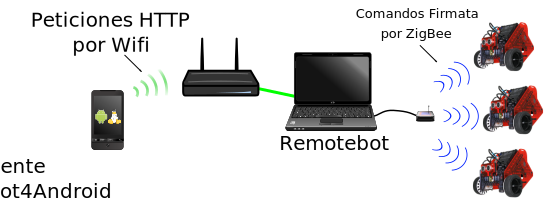
\includegraphics[width=\textwidth]{figures/arquitectura_remotebot}
    \caption{Esquema de conexión de RemoteBot}\label{fig:arquitectura_remotebot}
\end{figure}



Remotebot provee una API JSON a través de HTTP que permite controlar a los
robots de forma remota. Pero si bien es posible poner el servicio público,
el mismo no cuenta con autenticación, no soporta bien la concurrencia
y no provee ningún mecanismo de seguridad por lo que es recomendable solamente
usarlo dentro de ámbito de una red LAN.
La implementación del servidor
usa el módulo ``SimpleHTTPServer'' de la biblioteca estándar de Python para
proveer el soporte del protocolo HTTP e
introspección\footnote{\url{http://www.ibm.com/developerworks/library/l-pyint/}}.
para convertir los
mensajes enviados por los clientes en invocaciones a métodos.

\begin{figure}
    \centering
    \includegraphics[width=.5\textwidth]{figures/diagrama_remotebot}
    \subcaption{Diagrama de bloques de Remotebot}
    \label{fig:diagrama_remotebot}
\end{figure}
\begin{figure}
    \centering
    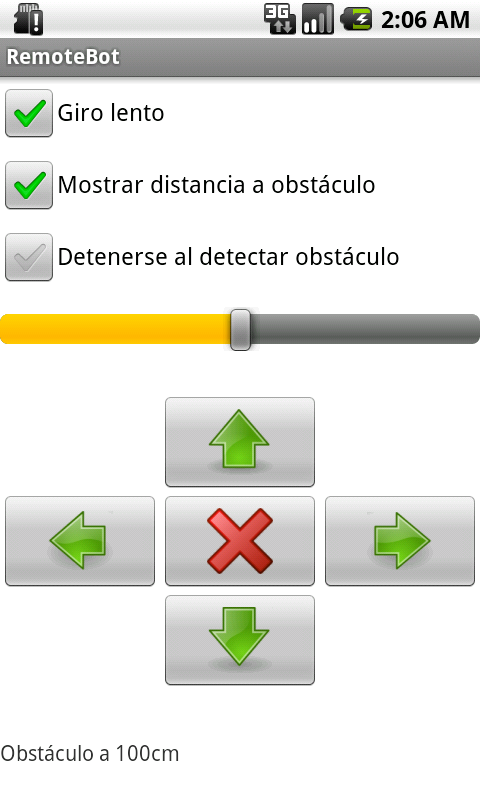
\includegraphics[width=.20\textwidth]{figures/cliente_remotebot}
    \subcaption{Cliente de Remotebot}
    \label{fig:cliente_remotebot}
\end{figure}

Si bien el servidor estaba diseñado para ser utilizado desde la
aplicación Android pedida por la materia,
se diseñó de forma tal de ser lo más genérico posible, dando acceso
a algunas caracterísiticas de DuinoBot no utilizadas por el cliente
Android como los sensores de línea con \texttt{getLine()} y operaciones
bloqueates como \texttt{forward(100, 1)} que no debe retornar
hasta pasado un segundo.

Como se ve en la figura~\ref{fig:diagrama_remotebot} Remotebot utiliza la
biblioteca DuinoBot para comunicarse con los robots y el cliente para el cuál
fue diseñado es una aplicación Android que permite controlar los robots
Multiplo N6
y ver los valores del sensor de distancia usando una interfaz con botones,
además de poder controlar el robot usando los acelerómetros del dispositivo
(inclinar el dispositivo en una dirección dada hace que el robot se mueva
en esa dirección).

Tanto el servidor RemoteBot como el cliente Remotebot4Android pueden
descargarse en
GitHub~\footnote{\url{https://github.com/fernandolopez/remotebot}}%
~\footnote{\url{https://github.com/fernandolopez/remotebot4Android}}.

\section{XRemoteBot}\label{sec:xremotebot}

La interacción de XRemoteBot a nivel arquitectura es muy similar a la
provista por Remotebot. La misma fue extendidad para
soportar robots Scribbler y puede ser
ampliada para interactuar con otros robots. Desde el punto de vista del cliente
XRemoteBot tiene varias diferencias, entre ellas la elección del protocolo,
usándose Websockets en lugar de peticiones HTTP y la definición del protocolo
de capa de aplicación que si bien es similar ahora posee un sistema de
autenticación opcional con una ``API key''.

% FIXME acá sé que falta más contenido del func. del servidor... (Fernando)

% FIXME donde estará el gráfico de esto?.
% me falta completar con la parte técnica de los módulos python
% usados, creo que algo de esto está escrito en otro capítulo
% lo tengo que pasar acá Fernando

\subsection{Configuraciones}

El servidor puede configurarse modificando el archivo
\texttt{xremotebot/configuration.py}. Como su nombre lo indica,
el archivo de configuración  es un archivo escrito en el lenguaje
Python por lo cuál cualquier modificación debe hacerse respetando
la sintaxis de este lenguaje.

Algunas de las variables de configuración que se pueden encontrar son:
\begin{itemize}
    \item \texttt{public\_server}: Es un booleano, si vale \texttt{True}
        el servidor requiere autenticación con una \textit{API key} para
        acceder a los robots, en cambio si vale \texttt{False} el servidor
        permite utilizar los robots sin solicitar una \textit{API key} y
        no utiliza el sistema de reservas por lo que cualquier usuario
        puede usar cualquier robot.
    \item \texttt{disable\_streaming}: Es un booleano, si vale \texttt{True}
        el servidor no hará streaming de video, ahorrando recursos tanto
        en el servidor como en los clientes que accedan a la interfaz Web,
        en cambio si vale
        \texttt{False} el streaming de video se encontrará habilitado
        y visible desde la interfaz Web.
    \item \texttt{robots}: Es un diccionario de Python, las claves
        deben ser modelos de robots soportados por XRemoteBot y por
        cada modelo debe tener como valor una lista con los identificadores
        de cada robot. Esta configuración determina el stock de robots
        disponibles a los que podrán acceder los usuarios.
    \item \texttt{hostname}: Es el nombre de dominio del servidor o bien
        su dirección IP.
    \item \texttt{port}: El puerto en el que esperará peticiones el
        servidor.
    \item \texttt{video\_ws}: Es la dirección y puerto del servidor de
        streaming de video utilizado. Normalmente la parte de
        dirección de esta configuración será igual a la variable
        \texttt{hostname}, pero se puede configurar de forma tal
        que el servidor de streaming esté en un servidor distinto
        al que provee la interfaz Web.
    \item \texttt{api\_key\_expiration}: Es un objeto de tipo fecha
        (\texttt{timedate}) que determina el tiempo de validez
        de las \textit{API keys}. Transcurrido este tiempo, el
        usuario deberá renovar su \textit{API key} para acceder
        a los robots.
    \item \texttt{reservation\_expiration}: Es un objeto de tipo
        fecha que determina la validez de las reservas de los robots.
        Una vez transcurrido este tiempo desde la reserva de un robot
        el usuario no podrá seguir usando este robot a menos que lo
        vuelva a reservarlo.
    \item \texttt{log\_file}: Es un string con el path donde se
        guardará el archivo de logs del servidor.
    \item \texttt{log\_level}: Es un string que determina en nivel
        de detalle a guardar en los logs. El valor puede ser
        cualquiera de los soportados por el módulo logging de
        Python\footnote{\url{https://docs.python.org/2/library/logging.html\#logging-levels}}.
\end{itemize}

La variable \texttt{robots} está intimamente
relacionada con la extensibilidad del servidor, ya que si por ejemplo
se quiere agregar soporte a XRemoteBot para manejar robots ``sphero''
basta con agregar la clave ``sphero'' al diccionario
\texttt{robots}. Si XRemoteBot encuentra la clave ``sphero'' en ``robots''
intentará cargar un plugin en el path
``remotebot/robots/sphero.py'',
el desarrollador debe implementar en este archivo una clase ``Robot''
que herede de ``remotebot.robots.abstract\_clases.Robot'' implementando
los métodos abstractos de esta clase.

Se puede ver un ejemplo de configuración del servidor en el
código~\ref{lst:config}. En este ejemplo el servidor cuenta
con cuatro robots utilizables, tres Multiplo N6 y un robot
Parallax Scribbler.

\begin{lstlisting}[language=python,
    caption={Configuración de ejemplo de XRemoteBot en
    \texttt{configuration.py}},
    label=lst:config]
tls = False
hostname = '190.16.204.135'                   # 'xremotebot.example'
video_ws = 'ws://{}:8084/'.format(hostname)
log_level = 'DEBUG'
log_file = 'remotebot.log'
port = 8000
public_server = False
api_key_expiration = days(700)
reservation_expiration = hours(1)
robots = {
    'n6': [13, 12, 11],
    'scribbler': ['00:1E:19:01:0B:81'],
}
\end{lstlisting}

% FIXME: Ampliar
% \chapter{WebSockets y Promises}\label{cha:websockets_y_promises}
% 
% Para el desarrollo de este trabajo decidió utilizar dos tecnologías
% que aún están en proceso de estandarización pero ya son ampliamente
% soportadas por distintos navegadores
% Web%
% ~\footnote{\url{http://caniuse.com/\#feat=websockets}}%
% ~\footnote{\url{http://caniuse.com/\#feat=promises}}
% como son la API
% \textit{WebSocket}~\footnote{La API en proceso de estandarización por la W3C,
% pero el protocolo ya fue estandarizado por IETF.}
% y la API \textit{Promise}~\footnote{En proceso de estandarización para
% ECMAScript 6 (Harmony).}.
% 
% En este capítulo se presenta una breve reseña de ambos y los motivos
% por los cuales fueron elegidos.

\subsection{WebSockets}\label{sec:websockets}

Para permitir el uso remoto de los robots a través de Internet sin necesidad
de requerir configuraciones ni puertos especiales se eligió implementar el
sistema como una
aplicación web. Sin embargo, como se menciona en el
capítulo~\ref{cha:protocolo} no se utiliza HTTP para el intercambio de
mensajes y valores de retorno entre los clientes y el servidor sino el
protocolo WebSocket.

El protocolo WebSocket permite mantener conexiones persistentes y no envía
encabezados HTTP en cada mensaje, reduciendo así el overhead en los mensajes
intercambiados que supondría el uso de HTTP~\citep{wang_2013}, aprovechando al
mismo tiempo los puertos TCP que abre el servidor Web.

La elección de este protocolo trae como desventaja frente al uso de HTTP la
necesidad de tener consideraciones de seguridad especiales. Para la parte
Web del sistema se utiliza autenticación con cookies pero no resulta seguro
utilizar el mismo mecanismo para la sesión con WebSockets ya que el sistema
quedaría vulnerable a ataques de tipo CSRF (Cross-Site Request
Forgery)~\citep{owasp_2014}~\footnote{
\url{https://www.owasp.org/images/5/52/OWASP_Testing_Guide_v4.pdf}}.

Una de las estrategias recomendadas es verificar el campo \texttt{Origin}
en los encabezados del hanshake inicial de WebSockets
desde el servidor, pero esta técnica no es suficiente ya que los
clientes pueden falsear este campo y solamente si el cliente es un navegador
envía este encabezado.
Otra estrategia es tener un mecanismo de autenticación
separado para la comunicación~\footnote{\url{https://www.christian-schneider.net/CrossSiteWebSocketHijacking.html}}.
Esta fue la estrategia elegida para XRemoteBot usando una \textit{API key}
para identificar a los usuarios al inicio de la comunicación.

\subsubsection{Otras alternativas a WebSockets}
Históricamente la forma de realizar requerimientos a un servidor desde un
cliente Javascript en un navegador fue usando la API
XMLHttpRequest\footnote{\url{http://www.w3.org/TR/XMLHttpRequest/}}, la
cual permite realizar peticiones HTTP sincronas y asincronas al
servidor\footnote{\url{https://developer.mozilla.org/en-US/docs/Web/API/XMLHttpRequest/Synchronous_and_Asynchronous_Requests\#Synchronous_request}}.

Este método cuenta con la desventaja de que en cada mensaje es necesario
enviar y recibir los encabezados HTTP y esto es muy costoso:
``Cada petición XHR es una petición individual HTTP y, en promedio, HTTP
tiene 800 bytes de sobrecarga (sin cookies HTTP) por cada
petición/respuesta''~\citep{grigorik_2013}.

Una posible solución a este problema es el uso de \textit{Long Polling},
uno de los ejemplos del uso de esta técnica es el protocolo \textit{Bayeux}
también conocido como \textit{Comet} por
su implementación principal
\textit{CometD}~\citep{roden_2010}. Bayeux puede funcionar con distintos
``transportes'', en particular CometD soporta ``long-polling'',
``callback-polling'' y WebSocket, en lo que resta de esta sección
consideraremos solamente los dos primeros.
El protocolo Bayeux permite al servidor demorar la respuesta
de ciertas peticiones, enviar al cliente respuestas incompletas para reutilizar
la conexión abierta en la petición o contestar varias peticiones de
una sola vez\footnote{\url{http://docs.cometd.org/3/reference/\#_bayeux}}.
Sin embargo cuando el cliente debe hacer una nueva petición enviará
nuevamente los encabezados HTTP e incluso el navegador puede llegar a
crear una nueva conexión TCP.

Otro uso de \textit{Long Polling} (probablemente el primer protocolo
de long polling definido) es el protocolo \textit{BOSH} que tiene
características similares a
Bayeux\footnote{\url{http://xmpp.org/extensions/xep-0124.html}}.

Si bien estos protocolos permiten evitar algunas reconexiones cuando
se trabaja de forma asincrónica con el servidor, eventualmente cuando el
servidor envíe una respuesta la conexión puede cerrarse la conexión TCP
si no hay tráfico en una determinada ventana de tiempo,
también cada mensaje
deberá tener su correspondiente encabezado HTTP, con lo cual
estas técnicas no resuelven completamente el problema del overhead del
uso de XMLHttpRequests sino que lo resuelven parcialmente y sobre todo
en aplicaciones asincrónicas donde se supone que el servidor puede enviar
datos al cliente en cualquier momento.

La elección de WebSockets resulta más natural para una implementación
como XRemoteBot ya que mantienen una conexión permantente y no intercambian
encabezados HTTP en cada mensaje (solamente un ``handshake'' inicial
al abrir la conexión).

